\subsection{Безынерционная модель}

% \subsection{Гипотеза о близости решений}
В литературе представлены \cite{Borisov2011, formalskii, ZobovaTatarinovPMM} работы, рассматривающие омниколеса в предположении, что массой и инерцией роликов можно пренебречь, налагающие на систему неголономные связи, ограничивающие направление скорости скольжения в точках контакта колес с поверхностью, на которой стоит экипаж, и не вводящие силу трения в контакте, т.е. считающие скольжение идеальным. Эти идеализированные модели имеют существенно меньше степеней свободы, чем "реальный" омниэкипаж, и легче поддаются аналитическому исследованию.

Описанные модели можно использовать для верификации построенной физически-ориентированной модели, рассматривая некоторые элементарные виды движений. Максимальное соответствие построенной модели упомянутым неголономным может быть достигнуто при уменьшении вляиния массы роликов на динамику колеса, а именно, при уменьшении их массы с сохранением общей массы колеса с роликами. На этом предположении и основан наш подход к верификации.

Для полноты коротко изложим результаты работы \cite{Borisov2011} как новейшей из неголономных моделей динамики свободной тележки с омниколесами на плоскости на момент выполнения работы.

Авторы \cite{Borisov2011} принимают простейшую модель омниколеса как плоского диска, для которого скорость точки контакта с опорной поверхностью направлена вдоль прямой, составляющей некоторый угол $\psi$ с плоскостью колеса (безынерционную модель, см. рис.~\ref{fig:bor_wheel_scheme}). Связь, наложенная на колесо в таком случае имеет вид
$$\vec{v_P}\cdot\vec{\mathbf{i}} = 0,$$
где $\vec{v_P}$ - скорость точки контакта $P$, $\vec{\mathbf{i}}$ - единичный вектор вдоль оси закрепления роликов.\\

\begin{figure}[ht!]
    \centering
    % 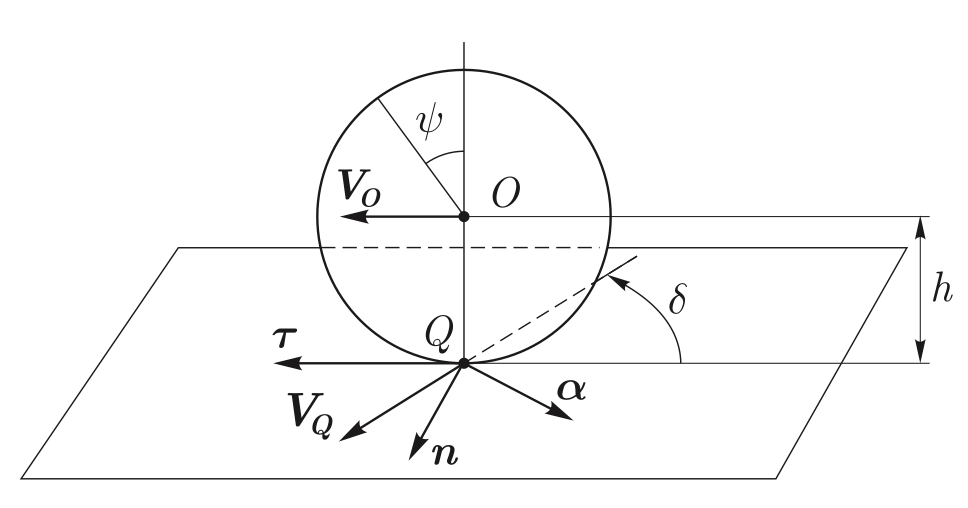
\includegraphics[width=0.75\textwidth]{content/parts/3_friction/diploma/img/art/bor_wheel_scheme.png}
    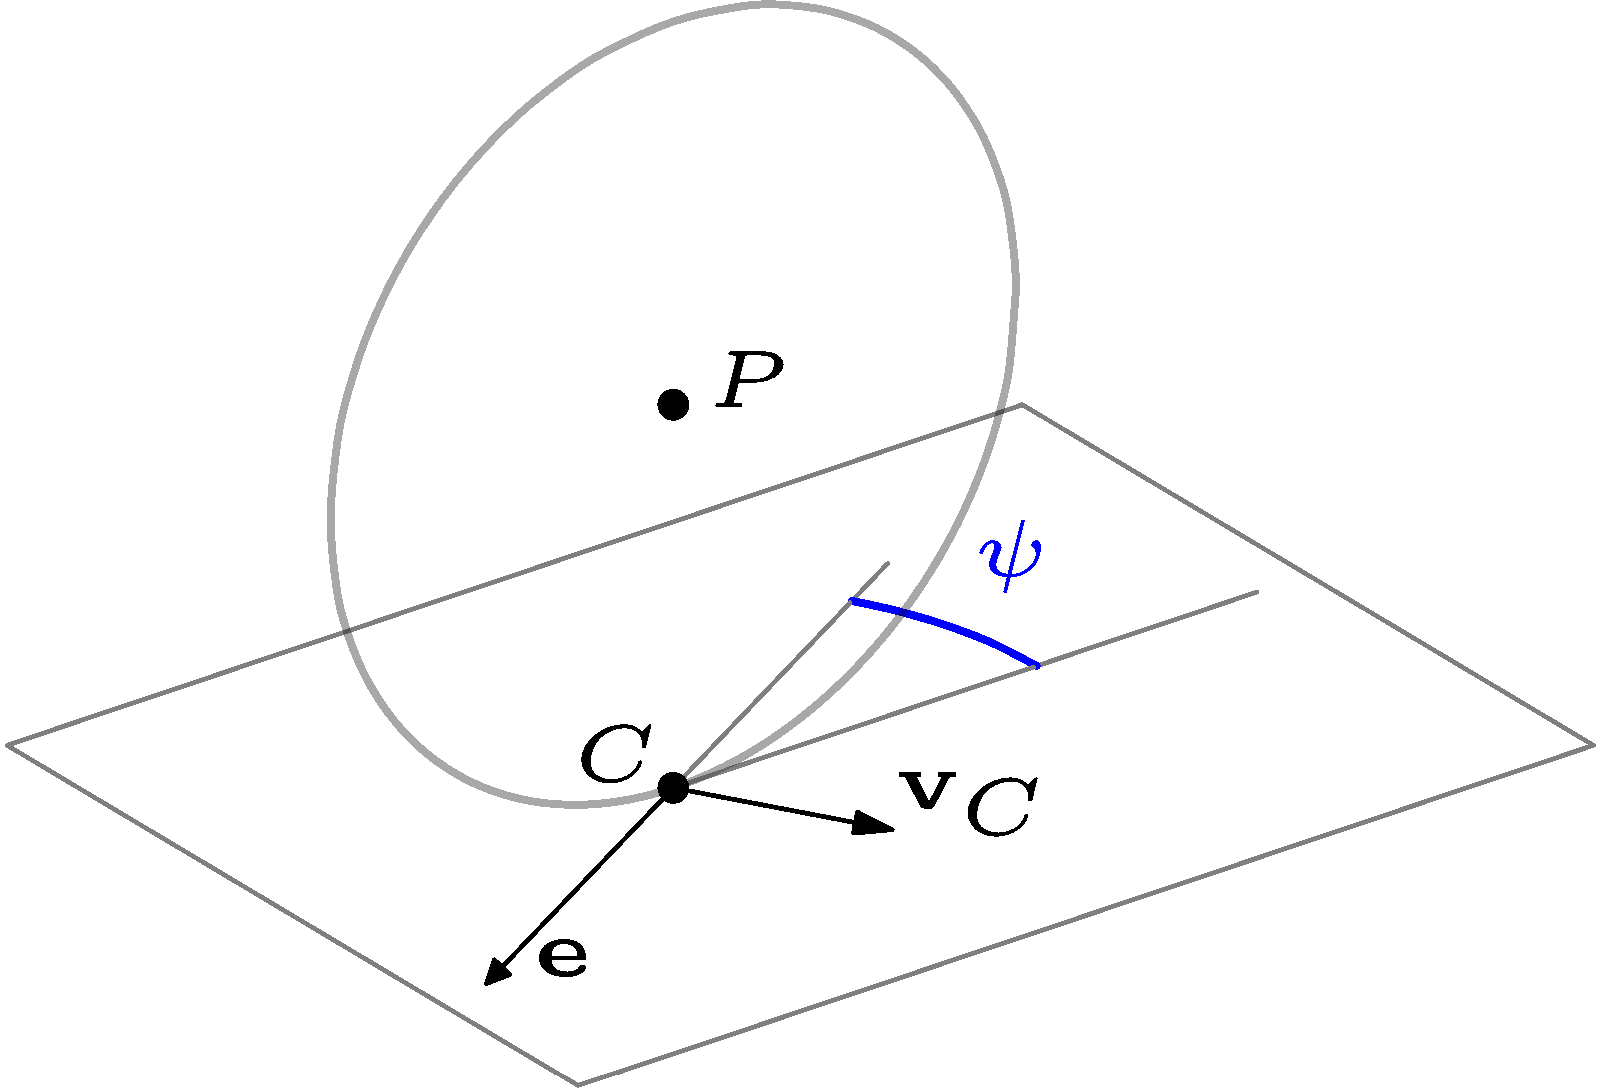
\includegraphics[width=0.5\textwidth]{content/pic/asy/wheel_bor.png}
    % \asyinclude[width=0.75\textwidth]{content/pic/asy/wheel_bor}
    \caption{Безынерционная модель колеса}
    \label{fig:bor_wheel_scheme}
\end{figure}

Авторы \cite{Borisov2011} получают уравнения движения для экипажа с произвольным количеством колес, закрепленных так, что их оси неподвижны относительно платформы, а оси роликов повернуты на произвольные углы относительно плоскостей соответствующих колес (см. фиг.~\ref{fig:bor_vehicle}).

\begin{figure}[ht!]
    \centering
    % 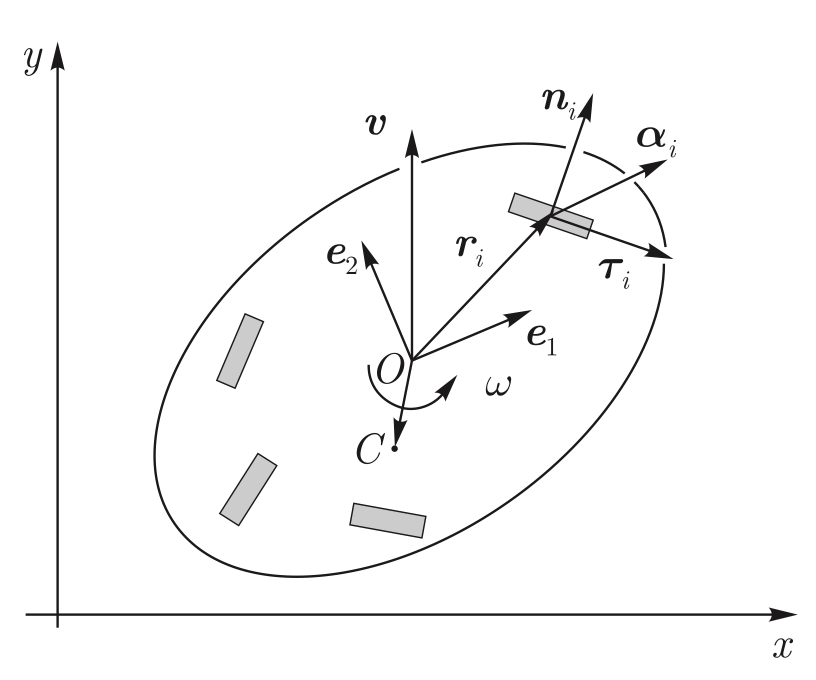
\includegraphics[width=0.75\textwidth]{content/parts/3_friction/diploma/img/art/bor_vehicle.png}
    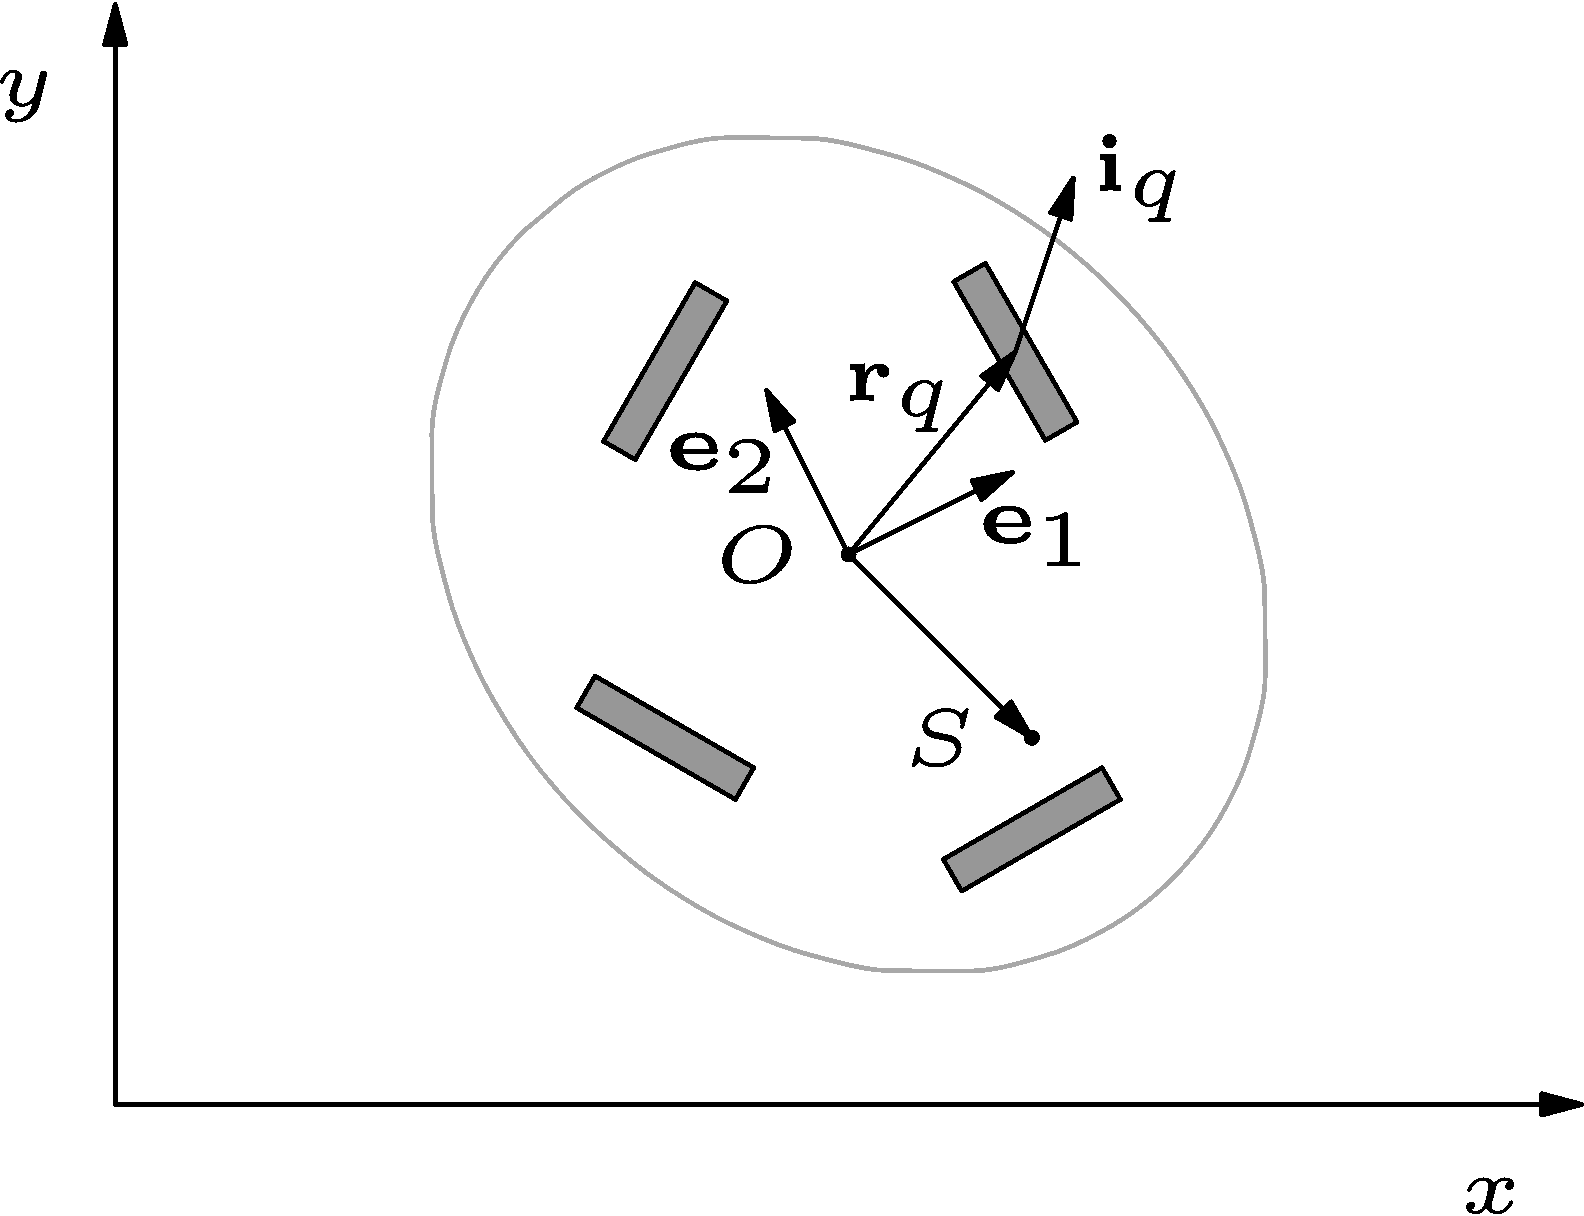
\includegraphics[width=0.75\textwidth]{content/pic/asy/cart_bor.png}
    \caption{Безынерционная модель экипажа}
    \label{fig:bor_vehicle}
\end{figure}

Вводится подвижная система отсчета $O\vec{e}_1\vec{e}_2$, связанная с платформой экипажа. Уравнения свободного движения имеют вид:
\begin{eqnarray*}
    (\Gamma+mE)\dot{\vec{v}}_O + m\dot{\omega}(J\vec{r}_S+\vec{R}_O)+m\omega J(\vec{v}_O + \omega J\vec{r}_S) = 0,\\
    \hat{I}\dot{\omega} + m(J\vec{r}_S+\vec{R}_O)\cdot\dot{\vec{v}}_O+m\omega\vec{v}_O\cdot\vec{r}_S = 0,\\
    \dot{x} = v_1\cos\phi - v_2\sin\phi, \quad \dot{y} = v_1\sin\phi + v_2\cos\phi, \quad \dot{\phi} = \omega,\\
    \Gamma_{kl} = \sum_q \frac{I_q}{s_q^2 R_q^2}\vec{i}_q^k\vec{i}_q^l, \quad \vec{R}_O = m^{-1}\sum_q \frac{I_q}{s_q^2 R_q^2}(J\vec{r}_q\cdot \vec{i}_q) \vec{i}_q,\\
    \hat{I} = I + \sum_q \frac{I_q}{s_q^2 r_q}(J\vec{r}_q\cdot \vec{i}_q)^2,
\end{eqnarray*}
% \begin{eqnarray*}
% (\Gamma+mE)\dot{\vec{v}} + m\dot{\omega}(J\vec{r_C}+R)+m\omega J(\vec{v} + \omega J\vec{r_C}) = 0,\\
% \hat{I}\dot{\omega} + m(J\vec{r_C}+\vec{r})\cdot\dot{\vec{v}}+m\omega\vec{v}\cdot\vec{r_C} = 0,\\
% \dot{x} = v_1\cos\phi - v_2\sin\phi, \dot{x} = v_1\sin\phi + v_2\cos\phi, \dot{\phi} = \omega,\\
% \Gamma_{kl} = \sum_i \frac{I_i}{s_i^2 h_i^2}\alpha_i^k\alpha_i^l, R = m^{-1}\sum_i \frac{I_i}{s_i^2 h_i^2}(J\vec{r_i}\cdot \alpha_i) \alpha_i,\\
% \hat{I} = I + \sum_i \frac{I_i}{s_i^2 h_i}(J\vec{r_i}\cdot \alpha_i)^2,
% \end{eqnarray*}
\newline
где $\hat{I}$ - суммарный момент инерции системы относительно вертикальной оси, проходящей через начало $O$ подвижной системы отсчета,\newline
$I$ - момент инерции платформы относительно той же прямой,\newline
$I_i$ - моменты инерции колес относительно их диаметров,\newline
$s_q = \sin(\frac{\pi}{2} - \psi_q)$, \quad $R_q$ - радиусы колес,\newline
$\vec{r_q}$ - точки закрепления осей колес в подвижной системе,\newline
$J = \left(\begin{array}{cc}0 & 1\\-1 & 0\end{array}\right)$,
\quad $E$ - единичная матрица\newline
$x,y,\phi$ - координаты точки $O$ и угол поворота платформы экипажа вокруг вертикальной оси,\newline
$\vec{v}_O, \omega$ - вектор скорости точки $O$ и скорость поворота платформы,\newline
$\vec{r_S}$ - координаты центра масс экипажа в подвижных осях.

% Данная неголономная модель экипажа также реализована на языке Modelica \cite{ModelicaSpec} как часть упомянутой библиотеки \cite{KosenkoBond}. Таким образом, возможно проведение сравнительного анализа физически-ориентированной и идеализированной моделей и верифкация.

